\documentclass[]{article}
\usepackage{lmodern}
\usepackage{amssymb,amsmath}
\usepackage{ifxetex,ifluatex}
\usepackage{fixltx2e} % provides \textsubscript
\ifnum 0\ifxetex 1\fi\ifluatex 1\fi=0 % if pdftex
  \usepackage[T1]{fontenc}
  \usepackage[utf8]{inputenc}
\else % if luatex or xelatex
  \ifxetex
    \usepackage{mathspec}
    \usepackage{xltxtra,xunicode}
  \else
    \usepackage{fontspec}
  \fi
  \defaultfontfeatures{Mapping=tex-text,Scale=MatchLowercase}
  \setromanfont{TeX Gyre Pagella}
  \newcommand{\euro}{€}
\fi
% use upquote if available, for straight quotes in verbatim environments
\IfFileExists{upquote.sty}{\usepackage{upquote}}{}
% use microtype if available
\IfFileExists{microtype.sty}{%
\usepackage{microtype}
\UseMicrotypeSet[protrusion]{basicmath} % disable protrusion for tt fonts
}{}
\usepackage[margin=1in]{geometry}
\usepackage{graphicx}
\makeatletter
\def\maxwidth{\ifdim\Gin@nat@width>\linewidth\linewidth\else\Gin@nat@width\fi}
\def\maxheight{\ifdim\Gin@nat@height>\textheight\textheight\else\Gin@nat@height\fi}
\makeatother
% Scale images if necessary, so that they will not overflow the page
% margins by default, and it is still possible to overwrite the defaults
% using explicit options in \includegraphics[width, height, ...]{}
\setkeys{Gin}{width=\maxwidth,height=\maxheight,keepaspectratio}
\ifxetex
  \usepackage[setpagesize=false, % page size defined by xetex
              unicode=false, % unicode breaks when used with xetex
              xetex]{hyperref}
\else
  \usepackage[unicode=true]{hyperref}
\fi
\hypersetup{breaklinks=true,
            bookmarks=true,
            pdfauthor={M. Callaghan and V. Nieberg},
            pdftitle={Twitter and the European Hyperagora: What can the Twittersphere Tell us about Political Deliberation and Opinions in Europe?},
            colorlinks=true,
            citecolor=blue,
            urlcolor=blue,
            linkcolor=magenta,
            pdfborder={0 0 0}}
\urlstyle{same}  % don't use monospace font for urls
\usepackage{url}

\setlength{\parindent}{0pt}
\setlength{\parskip}{6pt plus 2pt minus 1pt}
\setlength{\emergencystretch}{3em}  % prevent overfull lines
\setcounter{secnumdepth}{0}

%%% Use protect on footnotes to avoid problems with footnotes in titles
\let\rmarkdownfootnote\footnote%
\def\footnote{\protect\rmarkdownfootnote}

%%% Change title format to be more compact
\usepackage{titling}

% Create subtitle command for use in maketitle
\newcommand{\subtitle}[1]{
  \posttitle{
    \begin{center}\large#1\end{center}
    }
}

\setlength{\droptitle}{-2em}
  \title{Twitter and the European Hyperagora: What can the Twittersphere Tell us
about Political Deliberation and Opinions in Europe?}
  \pretitle{\vspace{\droptitle}\centering\huge}
  \posttitle{\par}
  \author{M. Callaghan and V. Nieberg}
  \preauthor{\centering\large\emph}
  \postauthor{\par}
  \predate{\centering\large\emph}
  \postdate{\par}
  \date{October 23, 2015}



\begin{document}

\maketitle


{
\hypersetup{linkcolor=black}
\setcounter{tocdepth}{2}
\tableofcontents
}
\newpage

\section{Introduction}\label{introduction}

Twitter is an online social network that allows users to broadcast short
posts known as Tweets. Since its launch in 2006, the platform has
increasingly been used for everyday communication as well as for
political debates, crisis communication, marketing, and cultural
participation (Weller et al. 2013). The public-debt crisis in Europe is
widely discussed across Europe and presents an interesting point in time
to investigate whether European issues are discussed in a common
European public sphere. This project will do so by looking at data from
the communication platform Twitter. It will specifically look at the
reaction in the Twittersphere to the negotiation between the Troika and
Greece leading up to the signing of the three memorandums.

\section{Research Question}\label{research-question}

In our research project we will investigate the following questions:

What can twitter tell us about pan-European reactions to the European
governance of the public-debt crisis in Greece?

\begin{itemize}
\item
  What can variation across time and space in the volume of Tweets
  regarding the euro crisis tell us about popular engagement with the
  issues?
\item
  What can the content of Tweets related to the crisis tell us about the
  spread of public opinion on the handling of the crisis in Greece
  between and within countries?
\end{itemize}

By investigating European public discourse on the Euro crisis the answer
to these questions could potentially add to the literature on the
emergence of a European public sphere.

\section{Literature Review}\label{literature-review}

\subsection{On Twitter Research}\label{on-twitter-research}

The body of twitter research has grown steadily in recent years (for a
comprehensive analysis and typology of twitter research up to 2013, see
Zimmer and Proferes 2014). Some of the findings relevant to our research
design are discussed below.

Twitter is a source of meaningful information about engagement with and
opinions about political topics. Twitter is also used as a platform for
political deliberation. In a recent study on Tweets mentioning parties
or politicians before the 2009 German federal election, Tumasjan et al.
found that ``Twitter is not just used to spread political opinions, but
also to discuss these opinions with other users'' (Tumasjan et al. 2010,
183). Furthermore, specific patterns of twitter usage have been
identifed that correspond with high-profile political events. Hughes and
Palen found that, compared to general Twitter usage, more
broadcast-based information sharing activities take place (Hughes and
Palen 2009, 259) during events. Moreover, Tumasjan et al. found that it
was possible to extact meaningful information about political opinions
from both the volumes and the content of these Tweets: ``the mere number
of Tweets reflects voter preferences and came close to traditional
election polls'' (Tumasjan et al. 2010, 183).

Twitter gives information on the location of Tweets and users, which
must be carefully interpreted. Devin Gaffney points out methodological
problems with using the given location of twitter users - ``in many
cases user-entered profile locations differ from the physical locations
users are actually Tweeting from'' (Graham, Hale, and Gaffney,Devin
2014, 1) which must be considered when interepreteing results.

Though the field of Sentiment Analysis (SA) is perhaps most developed in
the business world (Zimmer and Proferes 2014, 250), an increasing body
of literature has developed, focused on retrieving information about
political opinions from the Twittersphere. Though Tumasjan's results
have come under scrutiny (see Jungherr, J{ü}rgens, and Schoen 2012), the
authors found that ``the sentiment of Twiter messages closely
corresponded to political programs, candidate profiles, and evidence
from the media coverage of the campaign trail'' (Tumasjan et al. 2010,
183).

Grimmer provides an overview of recent developments in SA in political
science, noting how ``automated content methods can make possible the
previously impossible in political science: the systematic analysis of
large-scale text collections without massive funding support'' (Grimmer
and Stewart 2013, 2). He advises caution, however, about the utility of
SA in predictive models: ``The goal of building text models is therefore
different than model building to make causal inferences. {[}\ldots{}{]}
Emphasis in evaluations should be placed on helping researchers to
assign documents into predetermined categories, discover new and useful
categorizytion schemes for texts, or in measuring theoretically relevant
quantities from large collections of text.'' (Grimmer and Stewart 2013,
4).

Due to the enourmous amount of text available, Pak and Paroubek identify
that ``microblogging web-sites are rich sources of data for opinion
mining and sentiment analysis'' (Pak and Paroubek 2010, 1320). The
multilingual nature of Tweets across Europe presents some difficulties,
but is the subject of a growing body of research: ``Noisy social media,
such as Twitter, are especially interesting for sentiment analysis (SA)
{[}\ldots{}{]} given the amount of data and their popularity in
different countries, where users simultaneously publish opinions about
the same topic in different languages'' (Vilares, Alonso, and
G{ó}mez-Rodr{i}guez 2015, 2). Balahur and Turchi are confident about the
ability of Statistical Machine Translation (SMT) to provide a basis for
consistently applied SA across languages (Balahur and Turchi 2012, 58).
Other approaches include using emoticons to train models that assign
sentiment to a multilingual text corpus (Narr, Hulfenhaus, and Albayrak
2012).

Finally, some studies discuss ethical aspects of twitter research. For
example, concerns about creating a permanent archive of Tweets have been
voiced. These concerns included whether ``such archive was aligned with
users' privacy expectations'' (Zimmer and Proferes 2014, 258; Zimmer
2010).

\subsection{On Awareness and Public Opinion across Europe on the
Governance of the Public-Debt Crisis in
Greece}\label{on-awareness-and-public-opinion-across-europe-on-the-governance-of-the-public-debt-crisis-in-greece}

Academic research on the emergence of a European public sphere is not a
recent phenomenon (Risse 2003, 1). Hitherto, however, research has been
characterized as rather normative, as the ``research community has been
{[}\ldots{}{]} interested in producing policy recommendations for public
sphere-building'' (Trenz 2015, 234). Recent studies, on the other hand,
seem to put emphasis on an empirical grounding of the debate (Trenz
2015; Drewski, Gerhards, and others 2015). This development is being
mirrored in research on the public debate across Europe on the euro
crisis. It has been suggested that ``there is an emerging demos in the
European polity and it has been strengthened during the euro crisis''
(Risse 2014, 1213). When testing this hypothesis empirically, though, by
looking at newspaper editorials in Spain and Germany, Drewski found that
there were significant differences along national instead of ideological
lines in the discussion of the Euro crisis (Drewski, Gerhards, and
others 2015, 5).

Max Hänska and Stefan Bauchowitz in a recent LSE blog entry track
twitter activity during the negotiations leading up to the third Greek
bailout agreement. (Haenska and Bauchowitz 2015) According to their
findings, Tweets synchronised around key mini-events throughout the
negotiations, with peaks and troughs mirrored across national
twitter-spheres. These results suggest that popular engagement with the
issue converges across Europe.

\begin{figure}[htbp]
\centering
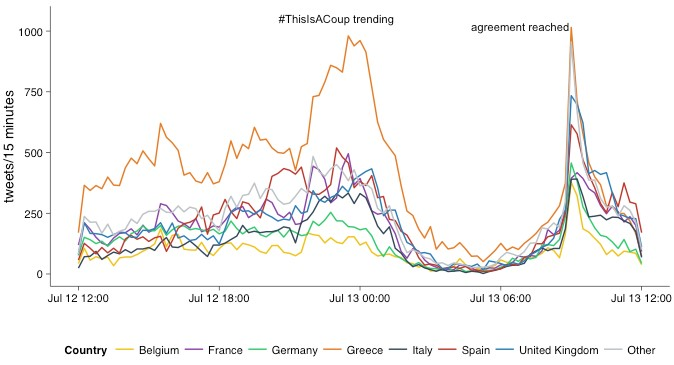
\includegraphics{img/Greece-twitter-1.jpg}
\caption{Tweet volumes by country on 12-13 July 2015 in European
countries (source Haenska and Bauchowitz 2015)}
\end{figure}

They further looked at instances of Tweets containing \#ThisIsACoup,
representing a particular opinion on the agreement. They then showed
that the spread of \#ThisIsACoup was not reflected in the studied
countries equally. This indicated a divergence of public opinion along
national lines.

\begin{figure}[htbp]
\centering
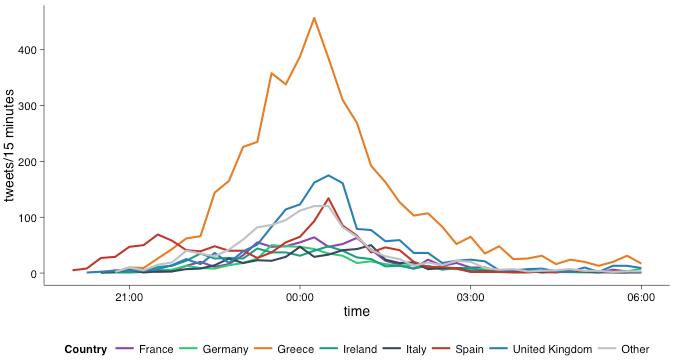
\includegraphics{img/Greece-twitter-2.png}
\caption{Number of Tweets containing the \#thisisacoup hashtag on 12-13
July 2015 (source Haenska and Bauchowitz 2015)}
\end{figure}

\section{Data Sources}\label{data-sources}

Two datasets are required for this project. The first is a corpus of
Tweets relating to the Greek debt crisis and the measures taken to
manage the crisis by European institutions. The second is information
about the users whose Tweets form the body of that corpus.

Zimmer and Proferes identify the Library of Congress' decision to place
every Tweet since Twitter's inception in 2006 into an archive as
validating ``the research importance of twitter'' (Zimmer and Proferes
2014, 251). Despite this announcement occuring in 2010, five years
later, the archive is still not open to researchers (Scola 2015).

Since late 2014, the whole corpus of twitter data has been searchable
online (Metz 2015). Programmatic access to this archive is, however,
more restricted. Twitter's public search API ``is not complete index of
all Tweets, but instead an index of recent Tweets. At the moment that
index includes between 6-9 days of Tweets.'' (``The Search API'' 2015).
Twitter sells access to historical Tweets through an API provided by its
``enterprise API platform'' GNIP (Tornes 2015). This paper will adapt a
publicly available program written in Java which scrapes results from
Twitter's online search page (Henrique 2015). A list of queries
involving combinations of keywords to do with the Greek debt crisis will
be drawn up, and we will programmatically run through the list, using
the GetOldTweets software to scrape the Tweets returned by Twitter's
comprehensive online search function that are given by each query.

We can use the R package `TwitteR' (Gentry 2015) to retrieve more
information about the unique users in our corpus dataset. The two
datasets can then be merged so that Tweets can be mapped by location.

\section{Methodology}\label{methodology}

\begin{itemize}
\item
  Volumes of topic-relevant Tweets will be mapped across space and time,
  to analyse the distribution of topic-awareness and its relation to
  political developments in responses to the crisis.
\item
  The distribution of hashtags that clearly represent an opinion on the
  response to the crisis (e.g. `\#ThisIsaCoup', `\#ThisIsNotaCoup'
  \emph{inter alia}) will be similarly mapped in order to approximate
  the distribution of opinion within and between countries over time.
\item
  The paper will attempt a sentiment analysis of Tweets expressing
  opinions about the agreed bailout deals using either/or/a combination
  of:

  \begin{itemize}
  \item
    A multilingual EU funded open-source sentiment analysis tool
    (opeNER)
  \item
    Machine translation to translate all texts into English before
    performing sentiment analysis
  \item
    Sentiment analysis based on emoticons
  \end{itemize}
\end{itemize}

Option two will be preferred, due to simplicity, and analysis will then
be carried out using unigrams to indicate polarity through comparison
with a lexicon. Following Grimmer, ``We will assume documents are a
\emph{bag of words}, where order does not inform our analyses'' as ``In
practice, for common tasks like measuring sentiment, topic modeling, or
search, \emph{n-grams} (combinations of words rather than individual
words) do little to enhance performance'' (Grimmer and Stewart 2013, 6).

Based on the results of sentiment analysis carried out and analysis of
volumes of tweets and users using opinion-signifying keywords, the paper
will give an indication of the scale of dialogue, consensus and
disagreement across and within countries in the European Twittersphere.

\section*{References}\label{references}
\addcontentsline{toc}{section}{References}

Balahur, Alexandra, and Marco Turchi. 2012. ``Multilingual Sentiment
Analysis Using Machine Translation?'' \emph{Proceedings of the 3rd
Workshop in Computational Approaches to Subjectivity and Sentiment
Analysis P. 52-60}.
\url{http://publications.jrc.ec.europa.eu/repository/handle/JRC73293}.

Drewski, Daniel, J{ü}rgen Gerhards, and others. 2015. ``Has There Been a
European Public Discourse on the Euro Crisis?''

Gentry, Jeff. 2015. \emph{TwitteR: R Based Twitter Client}.
\url{http://CRAN.R-project.org/package=twitteR}.

Graham, Mark, Scott a. Hale, and Gaffney,Devin. 2014. ``Where in the
world are you ? Geolocation and language identification in Twitter.''
\emph{The Professional Geographer} 00 (2013): 00.
doi:\href{http://dx.doi.org/10.1080/00330124.2014.907699}{10.1080/00330124.2014.907699}.

Grimmer, Justin, and Brandon M Stewart. 2013. ``Text as Data: The
Promise and Pitfalls of Automatic Content Analysis Methods for Political
Texts.'' \emph{Political Analysis}. SPM-PMSAPSA, mps028.

Haenska, Max, and Stefan Bauchowitz. 2015. ``A European Twitter Sphere?
What Tweets on the Greek Bailout Say About How Europeans Interact
Online.'' Accessed October 23. \url{http://perma.cc/6ZVZ-X5GT}.

Henrique, Jefferson. 2015. ``Get Old Tweets Programmatically.'' Accessed
October 21. \url{https://github.com/Jefferson-Henrique/GetOldTweets}.

Hughes, Amanda Lee, and Leysia Palen. 2009. ``Twitter adoption and use
in mass convergence and emergency events.'' \emph{International Journal
of Emergency Management} 6 (May): 248.
doi:\href{http://dx.doi.org/10.1504/IJEM.2009.031564}{10.1504/IJEM.2009.031564}.

Jungherr, Andreas, Pascal J{ü}rgens, and Harald Schoen. 2012. ``Why the
Pirate Party Won the German Election of 2009 or the Trouble with
Predictions: A Response to Tumasjan, a., Sprenger, tO, Sander, PG, \&
Welpe, IM `Predicting Elections with Twitter: What 140 Characters Reveal
About Political Sentiment'.'' \emph{Social Science Computer Review} 30
(2). SAGE Publications: 229--34.

Metz, Cade. 2015. ``Twitter Now Lets You Search for Any Tweet Ever
Sent.'' Accessed October 21.
\url{http://www.wired.com/2014/11/twitter-now-lets-search-tweet-ever-sent}.

Narr, Sascha, Michael Hulfenhaus, and Sahin Albayrak. 2012.
``Language-Independent Twitter Sentiment Analysis.'' \emph{Knowledge
Discovery and Machine Learning (KDML), LWA}, 12--14.

Pak, Alexander, and Patrick Paroubek. 2010. ``Twitter as a Corpus for
Sentiment Analysis and Opinion Mining.'' \emph{In Proceedings of the
Seventh Conference on International Language Resources and Evaluation},
1320--26.
doi:\href{http://dx.doi.org/10.1371/journal.pone.0026624}{10.1371/journal.pone.0026624}.

Risse, Thomas. 2003. ``An Emerging European Public Sphere? Theoretical
Clarifications and Empirical Indicators.''

---------. 2014. ``No Demos? Identities and Public Spheres in the Euro
Crisis.'' \emph{JCMS: Journal of Common Market Studies} 52 (6):
1207--15.
doi:\href{http://dx.doi.org/10.1111/jcms.12189}{10.1111/jcms.12189}.

Scola, Nancy. 2015. ``Library of Congress' Twitter Archive Is a Huge
\#FAIL.'' Accessed October 23.
\url{http://www.politico.com/story/2015/07/library-of-congress-twitter-archive-119698.html}.

``The Search API.'' 2015. https://dev.twitter.com/rest/public/search.
Accessed October 21.

Tornes, Adam. 2015. ``Instant and Complete Access to Every Historical
Public Tweet.''
\url{https://blog.twitter.com/2015/full-archive-search-api}.

Trenz, Hans-Jörg. 2015. ``Europeanising the Public Sphere -- Meaning,
Mechanisms, Effects.'' In \emph{Interdisziplinäre Europastudien}, edited
by Ulrike Liebert and Janna Wolff, 233--51. Springer Fachmedien
Wiesbaden.
doi:\href{http://dx.doi.org/10.1007/978-3-658-03620-1_11}{10.1007/978-3-658-03620-1\_11}.

Tumasjan, Andranik, Timm Oliver Sprenger, Philipp G Sandner, and Isabell
M Welpe. 2010. ``Predicting Elections with Twitter: What 140 Characters
Reveal About Political Sentiment.'' \emph{ICWSM} 10: 178--85.

Vilares, David, Miguel A Alonso, and Carlos G{ó}mez-Rodr{i}guez. 2015.
``Sentiment Analysis on Monolingual, Multilingual and Code-Switching
Twitter Corpora.'' In \emph{6TH WORKSHOP oN COMPUTATIONAL APPROACHES tO
SUBJECTIVITY, SENTIMENT aND SOCIAL MEDIA ANALYSIS WASSA 2015}, 2.

Weller, Katrin, Axel Bruns, Jean Burgess, Merja Mahrt, and Cornelius
Puschmann. 2013. \emph{Twitter and Society}. Vol. 89. Peter Lang New
York.

Zimmer, Michael. 2010. ``Is It Ethical to Harvest Public Twitter
Accounts Without Consent?''
\url{http://www.michaelzimmer.org/2010/02/12/is-it-ethical-to-harvest-public-twitter-accounts-without-consent/}.

Zimmer, Michael, and Nicholas John Proferes. 2014. ``A topology of
Twitter research: disciplines, methods, and ethics.'' \emph{Aslib
Journal of Information Management} 66 (3): 250--61.
doi:\href{http://dx.doi.org/10.1108/AJIM-09-2013-0083}{10.1108/AJIM-09-2013-0083}.

\end{document}
